\subsubsection{Sensores rotativos} \mbox{} \vspace{10pt} \\
Un sensor es un dispositivo eléctrico y/o mecánico capaz de convertir magnitudes físicas, como la luz, velocidad, aceleración, presión, temperatura, etc. En otra magnitud, normalmente eléctrica, que sea posible manipular y cuantificar.

Para nuestro caso en particular, usamos los sensores para medir la velocidad de los motores. Como el objetivo es construir un sistema de lazo cerrado que controle la velocidad de los motores con el fin de aproximar la trayectoria calculada.

Para medir la velocidad en revoluciones por minuto (RPM), se colocó, en el eje del motor, una rueda con patrón impreso el cual es detectado por un sensor infrarrojo (opto acoplador de ranura). El patrón impreso consta de líneas perforadas, ranuras, en la rueda con el fin de generar interrupciones. Se realizaron 24 ranuras en cada rueda para poder realizar el cálculo de la distancia recorrida.

Para realizar la medición de RPM se experimentó tres métodos diferentes:

\begin{itemize}
   \item Generando una interrupción con el flanco de señal obtenida del sensor infrarrojo. Las RPM se determinan en función de la cantidad de interrupciones contadas en el periodo de una base de tiempo implementada para este fin.
   \item Tomando el tiempo del sistema entre dos interrupciones consecutivas, y luego calcular las RPM.
   \item Midiendo la cantidad de pulsos generada por una base de tiempo externa entre dos interrupciones. Para lo cual se toma la lectura de un contador en la primera interrupción y se toma la lectura nuevamente en la interrupción siguiente. Con la diferencia entre las lecturas se calculan las RPM.
   \item Utilizando el contador de pulso incorporado en el microcontrolador ESP32, y para tener en cuenta las bajas revoluciones acumular los pulsos para luego calcular el promedio y obtener un resultado más preciso.
\end{itemize}

\begin{figure}[H]
  \centering
  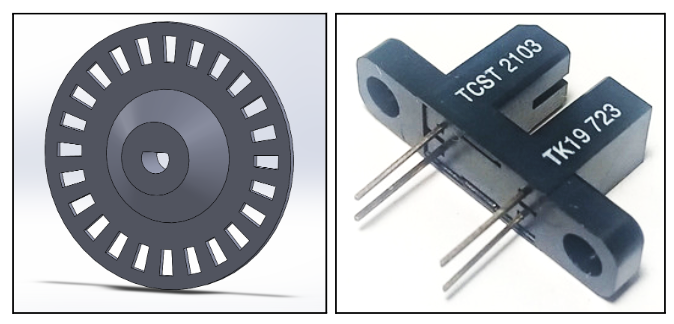
\includegraphics[width=0.7\linewidth]{images/encoder.png}
  \caption{Modelo 3D del encoder rotativo y opto acoplador de ranura}
  \label{fig:encoder}
\end{figure}

Por último se debe destacar que es necesario filtrar el rebote de los flancos de subida y bajada en cada interrupción.